\documentclass{ieeeaccess}

% xdvipdfmx (the XeTeX/Tectonic PDF driver) only picks up the class's
% \paperwidth/\paperheight from the second shipped page onward; without an
% explicit papersize special the first (title) page falls back to US Letter
% while every later page is the correct 203.2mm x 276.2mm IEEE Access size.
\special{pdf:pagesize width 203.2mm height 276.2mm}

\usepackage{cite}
\usepackage{amsmath,amssymb,amsfonts}
\usepackage{graphicx}
\usepackage{textcomp}
\usepackage{xcolor}
\usepackage{booktabs}
\usepackage{multirow}
\usepackage{url}
\usepackage[hidelinks]{hyperref}

\setlength{\textfloatsep}{6pt plus 2pt minus 2pt}
\setlength{\dbltextfloatsep}{6pt plus 2pt minus 2pt}
\setlength{\floatsep}{4pt plus 2pt minus 2pt}
\setlength{\intextsep}{6pt plus 2pt minus 2pt}
\setlength{\abovecaptionskip}{3pt}
\setlength{\belowcaptionskip}{2pt}

\def\BibTeX{{\rm B\kern-.05em{\sc i\kern-.025em b}\kern-.08em
    T\kern-.1667em\lower.7ex\hbox{E}\kern-.125emX}}

\begin{document}

\history{Date of publication xxxx 00, 0000, date of current version xxxx 00, 0000.}
\doi{10.1109/ACCESS.2026.0000000}

\title{Information-Matched Auditing of Conversational Emotion-Shift Forecasting}

\author{\uppercase{Bin Wen}\authorrefmark{1},
\uppercase{Dai-Qiao Zhang}\authorrefmark{2},
\uppercase{Tien-Ping Tan}\authorrefmark{1}}
\address[1]{School of Computer Sciences, Universiti Sains Malaysia, 11800 Gelugor, Penang,
Malaysia (e-mail: wenbin@student.usm.my; tienping@usm.my)}
\address[2]{School of Mathematical Sciences, Universiti Sains Malaysia, 11800 Gelugor, Penang,
Malaysia (e-mail: zhangdaiqiao24@student.usm.my)}
\tfootnote{This work was carried out using the authors' own computing resources; no external
funding was received for this research.}
\markboth{Wen \headeretal: Information-Matched Auditing of Conversational Emotion-Shift Forecasting}
{Wen \headeretal: Information-Matched Auditing of Conversational Emotion-Shift Forecasting}
\corresp{Corresponding author: Tien-Ping Tan (e-mail: tienping@usm.my).}

\begin{abstract}
Emotion-shift forecasting predicts whether the next conversational utterance will express a
different emotion before that utterance is observed. Comparisons are easily distorted when a
learned model receives rich features but its transition baseline is given a noisy or unavailable
current-emotion label, when hyperparameter budgets differ, or when target-turn information enters
the representation. We present an information-matched, leakage-safe audit with an explicit
commitment point, executable causality tests, equal four-configuration validation searches, and
seed--dialogue-aware inference. Six causal model families are evaluated on four text corpora and
two feature-source sensitivity configurations. In the deployable condition, a train-only current
emotion classifier feeds the transition baseline; in the oracle diagnostic, both learned models
and the baseline receive the same gold current emotion. Under the deployable condition, learned
models improve over the predicted-label transition baseline on all four primary text corpora;
DailyDialog gains are large and survive a 72-comparison Holm correction (best
$\Delta$ROC--AUC $=+0.167$, adjusted $p=.0144$). Under matched gold information, the transition
baseline remains competitive on IEMOCAP and is significantly stronger on MELD, whereas every
model retains a large DailyDialog advantage (best $\Delta=+0.132$, adjusted $p=.0144$). We also
report precision--recall AUC, calibration, a strictly utterance-local feature control,
same-person self-shift forecasting, and a same-architecture future-access dose response. The
results replace a binary ``model versus inertia'' narrative with a conditional one: conclusions
depend materially on current-label availability, corpus construction, target semantics, feature
provenance, and leakage discipline. Code, raw seed predictions, tests, and reporting artifacts
support reproducible auditing.
\end{abstract}

\begin{keywords}
emotion forecasting, conversational emotion recognition, evaluation protocol, data leakage, benchmarking
\end{keywords}

\titlepgskip=-21pt
\maketitle

\section{Introduction}

Consider a call-center assistant that flags, one turn before it happens, that a customer is about
to escalate from neutral to angry -- giving the agent seconds to change course. This is the promise
of \emph{forecasting} emotion in conversation, as opposed to \emph{recognizing} it: the target
state does not yet exist when the prediction is made. It is also precisely the setting in which a
model can look right without being right. If any feature -- a pooled dialogue embedding, a
bidirectional encoder, a context window one utterance too wide -- depends even slightly on the turn
being forecast, the model is not anticipating the future; it is reading it off a crib sheet built
into its own inputs. The failure is silent because nothing in a standard run signals it happened:
loss curves look normal, F1 looks respectable, the leaderboard entry looks like progress.

Emotion recognition in conversation (ERC) has a large, mature literature (\S II). A smaller but
growing thread reframes the task as forecasting -- predicting an upcoming emotional shift before
the triggering utterance is seen, the setting relevant to anticipatory dialogue systems,
de-escalation tools, and turn-taking agents. Forecasting is target-absent by construction: no
feature may depend on utterance $n{+}1$. This constraint is easy to violate silently, e.g.\ via
bidirectional encoders, dialogue-level pooling, or context windows not truncated at the decision
point -- and the architectures ERC has spent a decade refining are, almost without exception, built
to violate it, because recognition never had to enforce it in the first place.

We ask a measurement question: how do conclusions change when the future is actually hidden and
the learned model and transition baseline receive comparable current-state information? The two
requirements are distinct. A causal model without gold labels should be compared with a baseline
driven by train-only predicted labels; a baseline supplied with gold $y_n$ should be compared with
a model supplied with the same $y_n$. Our initial fixed-budget comparison confounded these regimes.
The present audit corrects that design, tunes every learned family with the same validation budget,
and propagates both dialogue and optimization uncertainty. The resulting picture is conditional
rather than uniformly negative: deployable models consistently improve on the predicted-label
baseline, while an information-matched oracle baseline remains hard on several corpora. Our
contribution is a measurement framework with six parts:

\begin{enumerate}
\item a formal commitment point and target-absent data construction for next-turn emotion shift;
\item an executable eight-item leakage audit plus future-perturbation causality tests;
\item train-only predicted-label and gold-label transition baselines that expose the information
available in each comparison;
\item equal four-configuration validation searches and checkpoint selection for six causal model
families, evaluated over three seeds;
\item seed--dialogue hierarchical intervals, paired dialogue-cluster permutation tests, and a
declared familywise Holm correction; and
\item provenance, future-access, and speaker-target controls that test whether conclusions survive
feature re-extraction, target redefinition, and controlled leakage.
\end{enumerate}

The final contribution matters because the two targets answer different questions. An
interaction-level system may legitimately care whether the \emph{conversation's} next turn changes
emotion regardless of who speaks. A coaching or wellbeing system may instead care whether the
\emph{same person} changes state when they next speak. Reporting one as if it were the other can
produce a semantically misleading claim even when the code is temporally leakage-free.

\section{Related Work}

\textbf{ERC backbones.} Our four ERC-derived models are representative of three context-modeling
paradigms: recurrent interlocutor-state tracking~\cite{majumder2019dialoguernn}, relational graph
convolution~\cite{ghosal2019dialoguegcn,ai2023dergcn}, and directed relational
attention~\cite{shen2021dagerc}. Knowledge-enriched encoders~\cite{zhong2019ket,ghosal2020cosmic}
and multimodal fusion architectures~\cite{tsai2019mult,hu2021mmgcn,hazarika2020misa,li2023ga2mif,meng2024mglra}
inform our feature choices (COSMIC RoBERTa; MM-DFN~\cite{hu2021mmdfn}-style
text+audio+visual). All are, in original form, bidirectional or graph-connected across the full
dialogue -- appropriate for recognition, but a direct leakage source if repurposed for forecasting
without a causal mask; interactive memory~\cite{hazarika2018icon} and contextual-reasoning
networks~\cite{hu2021dialoguecrn} share this property.

\textbf{Emotion forecasting (EFC).} A parallel line explicitly targets an unobserved future
utterance. Altarawneh et al.~\cite{altarawneh2023pec} formalize PEC as predicting turn $n{+}1$ from
context strictly up to $n$, decomposing the signal into sequence, self-dependency, and recency
terms (the strategy we re-implement as PEC-style, \S\ref{sec:exp}). Shi et
al.~\cite{shi2023epc,shi2024epc} model bilateral-speaker correlation and word-level cues in
text+audio. Hi-EF~\cite{wang2024hief} contributes a dedicated multimodal forecasting benchmark.
MREPC~\cite{ju2023mrepc} pre-trains contrastively over a short-term cross-speaker window.
PUGCN~\cite{xie2025pugcn} substitutes a pseudo-utterance-guided contrastive objective for the
absent target (the strategy behind our Pseudo-future-style re-implementation). EDFC~\cite{lu2023edfc}
targets a next-utterance emotion distribution; ERFC~\cite{debsharma2025erfc} shows feasibility in a
deployed call-center setting. All are cross-speaker by design and, to our knowledge, none audits a
leakage boundary as strict as ours. Notably EDFC and MM-DFN appeared at
ICASSP~\cite{lu2023edfc,hu2021mmdfn} and the EPC papers at Interspeech~\cite{shi2023epc,shi2024epc},
making this a speech-community concern as much as an NLP one.

\textbf{Emotion shift and flip: adjacent, not forecasting.} ESD-ERC~\cite{gao2022esderc},
CFN-ESA~\cite{li2024cfnesa}, and EmoShiftNet~\cite{nirujan2025emoshiftnet} use shift labels to
sharpen \emph{recognition} of an observed current utterance -- computed over turns the model can
already see. Emotion-flip reasoning~\cite{kumar2023efr,kumar2024ediref} runs backward: given a flip
that has already occurred, it attributes the past trigger. Neither predicts an unobserved future
shift under a leakage-safe protocol; we exclude both, noting our transition matrix is close in
spirit to the inertia signal they are designed to overcome.

\textbf{Leakage and baseline validity.} Kapoor and Narayanan~\cite{kapoor2023leakage} survey
at least 294 papers across 17 fields and find leakage the dominant cause of irreproducible
ML-based findings, proposing the taxonomy our 8-item audit is modeled after. Ferrari Dacrema et
al.~\cite{dacrema2019recsys} show most neural recommenders fail to beat tuned classical baselines
once evaluation is corrected; Lin~\cite{lin2019neuralhype} makes the same point for neural ranking.
We view our transition-matrix result as the same phenomenon in emotion forecasting.

\section{Task Definition and Threat Model}
\label{sec:task}

Let a dialogue be $D=\{(x_t,y_t,s_t)\}_{t=1}^{T}$, where $x_t$ is an utterance-level feature
vector, $y_t\in\{1,\ldots,K\}$ an emotion label, and $s_t$ a speaker identifier. At commitment
point $n$, a legitimate forecaster may use only
\begin{equation}
\mathcal{I}_n=\{x_{1:n},s_{1:n}\}\quad\text{and, when declared, }y_n,
\label{eq:info}
\end{equation}
but no quantity computed from $x_{n+1:T}$ or $y_{n+1:T}$. This definition includes an important
feature-provenance condition: $x_t$ must itself be utterance-local. Merely slicing a dialogue-level
bidirectional representation at index $n$ does not make it causal.

\subsection{Two Forecasting Targets}

Our original and primary target is the \emph{interaction-level immediate shift}
\begin{equation}
z_n^{\mathrm{int}}=\mathbb{1}[y_{n+1}\neq y_n],\qquad n<T.
\label{eq:interaction}
\end{equation}
It is operationally appropriate when the question is ``will the emotion expressed in the next
turn differ from the emotion expressed now?'' It is agnostic to speaker identity and therefore
mixes two strata: $s_{n+1}=s_n$ and $s_{n+1}\neq s_n$.

For semantic clarity we additionally define the \emph{next-own-utterance self-shift}. Let
\begin{equation}
g(n)=\min\{m>n:s_m=s_n\}
\end{equation}
when such an utterance exists. Then
\begin{equation}
z_n^{\mathrm{self}}=\mathbb{1}[y_{g(n)}\neq y_n].
\label{eq:self}
\end{equation}
This target asks whether the current speaker changes emotion by the time they next speak, allowing
intervening turns by others. It removes the immediate cross-speaker label comparison, but it is not
``more correct'' in the abstract: it answers a different product and scientific question, has a
variable forecast horizon, and excludes terminal appearances of each speaker. We report both rather
than silently substituting one for the other.

\subsection{What Counts as Leakage?}

Table~\ref{tab:threats} distinguishes information leakage from other sources of optimistic or
misleading evidence. The first three rows violate Eq.~\eqref{eq:info}; the remaining rows do not
necessarily leak the future but can still make comparisons invalid. This separation prevents the
term ``leakage'' from becoming a catch-all diagnosis.

\begin{table*}[t]
\centering
\footnotesize
\caption{Threat model for conversational emotion forecasting. The audit treats target-derived
features and target-derived model states as zero-tolerance failures; the other threats require
separate statistical or reporting controls.}
\label{tab:threats}
\begin{tabular}{p{0.17\textwidth}p{0.29\textwidth}p{0.24\textwidth}p{0.20\textwidth}}
\toprule
Threat & Failure mechanism & Detection & Required control \\
\midrule
Target-turn exposure & $x_{n+1}$ enters a window, pooled context, or auxiliary input & inspect
window boundaries; sweep visible future turns & truncate at $n$ before any aggregation \\
Bidirectional state & output at $n$ depends on representations from $n+1:T$ & perturb future
inputs and compare prefix logits & unidirectional recurrence or explicit causal mask \\
Feature provenance & nominally per-turn $x_n$ was extracted with dialogue-level future context &
trace the feature extractor, not only the classifier & utterance-local extraction or causal
re-extraction \\
Split contamination & duplicate dialogue text or the same global speaker occurs across folds &
hash dialogue text; audit global identities & group-aware split and duplicate removal \\
Selection leakage & test fold determines threshold, epoch, or model family & inspect tuning log &
validation-only selection with fixed test evaluation \\
Metric degeneracy & high base rate makes always-shift F1 look competitive & report prediction
rate and balanced metrics & AUC, balanced accuracy, and constant baselines \\
Semantic target drift & cross-speaker next-turn change is described as same-person emotional change
& stratify by $s_{n+1}=s_n$; evaluate Eq.~\eqref{eq:self} & name the target and deployment contract \\
\bottomrule
\end{tabular}
\end{table*}

\section{Protocol}

\textbf{Commitment point.} For decision point $n$, all input features (text/audio/visual) are
restricted to utterances $\leq n$; the target label is $\mathbb{1}[y_{n+1} \neq y_n]$. All six
learned models (\S\ref{sec:exp}) are structurally causal, not causal-by-convention.

\textbf{Information-matched regimes.} In the \emph{deployable} regime, learned models receive
utterance features and causal history but no gold emotion label. The transition baseline instead
uses $\hat y_n$ from a linear current-emotion classifier fit exclusively on training utterances;
its regularization is selected on the validation fold. In the \emph{oracle diagnostic}, the gold
one-hot $y_n$ is appended to every learned model and the transition baseline conditions on the same
gold $y_n$. This is not a deployment claim: it isolates the value of forecasting beyond a shared,
perfect observation of current state. Comparing a no-label model only against a gold-label
transition matrix is retained as a useful stress test, but is not used as the deployable headline.

\textbf{Causal construction and a zero-tolerance check.} DialogueRNN's global/party/emotion states
update by chained \texttt{GRUCell} calls that never touch $x_{t+1:}$. DialogueGCN uses
\emph{windowed} causal edges ($j{\to}i$ iff $j\leq i$ and $i-j\leq 6$); DAG-ERC uses
\emph{unbounded} causal attention ($j\leq i$, any distance) -- two families differing sharply in
receptive field yet still landing within the same $\lesssim$0.04 AUC band (\S\ref{sec:exp}), which
strengthens rather than weakens Finding 4. We verified causality directly rather than trusting
architecture alone: perturbing every input at $t\geq n$ to random noise leaves outputs at $t<n$
changed by exactly 0.0 (floating-point identical) for every model.

\textbf{Automated leakage audit.} Every experiment emits an 8-item checklist: last-utterance
masking, model causality, per-utterance feature scope, speaker-split disjointness, val-only threshold
tuning, dialogue-level bootstrap, train-fold-only baseline fitting, and baseline completeness.

\textbf{Padding and supervision masks.} Dialogue batches are right padded, but the final true
utterance of every dialogue and every padded position receive an ignore label. Classification loss,
threshold selection, and metrics operate only on valid decision points. For the corrected
Pseudo-future implementation, its auxiliary next-embedding regression is masked by the same valid
decision-point tensor. This detail matters because unmasked padding creates a length-dependent
training signal even though it does not directly expose the future.

\textbf{Strong baseline.} Beyond base-rate and no-change/inertia, we fit a
speaker$\times$emotion transition matrix $P(y_{n+1} \mid y_n, \text{speaker})$ on the train fold
only (Laplace $\alpha{=}1.0$; a speaker's row is used only with $\geq$20 training observations,
else global backoff). This is the baseline every model must beat.

\textbf{Equal validation budget.} Each architecture receives the same four candidates spanning
hidden size $\{64,128,256\}$, learning rate $\{3\!\times\!10^{-4},10^{-3}\}$, dropout
$\{.1,.3\}$, and focal versus class-balanced cross-entropy loss. Seed 0 is used for configuration
selection on validation ROC--AUC only. The selected configuration is then trained with seeds
$\{0,1,2\}$ for at most 30 epochs; the validation-selected checkpoint uses a five-epoch patience
after at least five epochs. The test fold is never evaluated during search or checkpoint
selection. A validation-selected binary threshold affects only thresholded metrics, not ROC--AUC,
PR--AUC, Brier score, or calibration error.

\textbf{Metrics.} ROC--AUC is primary because it is threshold-free. We additionally report
PR--AUC for the imbalanced shift class, Brier score and expected calibration error, shift-F1,
precision, recall, and balanced accuracy. Predictors assigning more than 98\% of decisions to one
class are automatically flagged. PR--AUC is interpreted relative to each corpus's shift prevalence,
not compared naively across corpora~\cite{saito2015pr}; calibration is measured on probabilities,
separately from discrimination~\cite{guo2017calibration}.

\textbf{Significance.} Differences are estimated with a hierarchical bootstrap~\cite{saravanan2020bootstrap}
that first samples
training seeds and then resamples whole test dialogues ($1{,}999$ replicates). Two-sided paired
dialogue-cluster permutation tests use $4{,}999$ sign flips and the plus-one correction, so a
reported $p$-value is never zero. Holm--Bonferroni correction is applied jointly across the two
information regimes, six models, and six dataset-configurations (72 declared comparisons).

\textbf{Reproducibility contract.} Random seeds are fixed at 0, 1, and 2. Each dataset is loaded
and split before model construction; no fitted current-emotion classifier or cached prediction is
shared across seeds. Raw scores for every seed are retained and jointly enter inference. Dataset
manifests record SHA-256 hashes, split identifiers are deterministically ordered, and independent
tests verify that perturbing inputs at and after the forecast boundary cannot alter earlier logits.
DailyDialog validation/test dialogues exactly duplicated in training are removed before any search.

\section{Experiments}
\label{sec:exp}

\textbf{Data.} The primary analysis uses four text corpora with released RoBERTa features
(IEMOCAP~\cite{busso2008iemocap}, MELD~\cite{poria2019meld}, EmoryNLP~\cite{zahiri2018emorynlp},
DailyDialog~\cite{li2017dailydialog}; COSMIC pipeline~\cite{ghosal2020cosmic}), plus two multimodal
configurations (IEMOCAP, MELD with MM-DFN~\cite{hu2021mmdfn}
text+OpenSmile-audio+DenseNet-visual features) are reported only as feature-source sensitivity
analyses because the available release does not include the complete upstream extraction code.
Table~\ref{tab:stats} gives size and shift-rate statistics (0.20--0.72) together with an
F1-degeneracy analysis referenced below.

The six configurations are not six independent corpora: IEMOCAP and MELD each appear once with
COSMIC text features and once with MM-DFN multimodal features. This paired reuse is intentional for
the feature-source comparison, but inferential claims are made per configuration and are not
treated as six independent replications. COSMIC features are 1024-dimensional RoBERTa vectors;
MM-DFN provides 600/100-dimensional text, 300/1582-dimensional audio, and 342-dimensional visual
vectors for MELD/IEMOCAP, respectively. We use official or released train/test identifiers;
MM-DFN lacks validation identifiers, so a deterministic 10\% slice of the training dialogues is
reserved for validation. We verified the released COSMIC producer scripts for IEMOCAP, MELD, and
EmoryNLP and confirmed that the stored RoBERTa rows are generated per utterance. As an independent
control that does not rely on released embeddings, we also fit TF--IDF vocabulary/IDF and truncated
SVD on training utterances only and transform every utterance independently. DailyDialog contains
134 test and 101 validation dialogues exactly duplicated in training; all revised DailyDialog
results remove those dialogues before configuration selection or evaluation.

\subsection{Compared Models}

The benchmark spans recurrence, structured speaker state, graph propagation, directed attention,
and two forecasting-specific strategies. To keep the question focused on the temporal contract,
each model maps the same feature sequence to one logit per observed turn and uses the same loss and
optimization budget. DialogueRNN maintains global and party states; causal DialogueGCN propagates
messages only from earlier nodes in a six-turn window; DAG-ERC uses unbounded causal attention;
PEC-style concatenates sequence, self-dependency, and exponentially weighted recency states; and
Pseudo-future-style predicts an embedding for $x_{n+1}$ from the causal state before classifying
shift. The actual $x_{n+1}$ is only an auxiliary regression target during training and never a
forward-path input.

\textbf{State-factorized control.} Shift-only supervision collapses every directed emotion
transition to one bit. Motivated by work that predicts the next-utterance emotion distribution
directly~\cite{lu2023edfc}, we add a causal multi-task control with three heads: current emotion,
future emotion, and direct shift. Its factorized shift probability is
$1-\sum_k p(y_n{=}k\mid\mathcal I_n)p(y_{n+1}{=}k\mid\mathcal I_n)$; a convex blend with the
direct head is selected on validation data only. No gold label or future utterance enters inference.
Because this model was designed after the audit, it is evaluated in a separately declared
four-corpus family rather than inserted post hoc into the 72 main comparisons. It reaches
.628/.628/.546/.747 ROC--AUC on IEMOCAP/MELD/EmoryNLP/DailyDialog and improves over the deployable
transition baseline by +.052/+.041/+.043/+.166; MELD and DailyDialog remain significant after
four-test Holm correction ($p=.0036$ and $.0008$). Its score is comparable to, rather than higher
than, the best main-benchmark architecture.

We also retain a bidirectional GRU solely as a positive leakage control. It is not a candidate
forecaster. Its purpose is diagnostic: if the safe and leaky models perform identically, either the
target utterance carries little useful signal or the benchmark implementation is failing to learn;
if the leaky model improves sharply, the latter explanation becomes less plausible.

\begin{table}[t]
\centering
\footnotesize
\caption{Dataset statistics and F1 degeneracy. Always-shift F1 $=2r/(1{+}r)$ for shift rate $r$
(analytic; always-shift balanced accuracy is 0.500 by construction, omitted). Transition-BA
$\approx$0.50 on MELD/EmoryNLP/IEMOCAP-mm shows standard F1 sits at the degenerate ceiling on
exactly the corpora where shift is common; only IEMOCAP and DailyDialog clear it.}
\label{tab:stats}
\resizebox{\linewidth}{!}{%
\begin{tabular}{lrrrcc}
\toprule
Dataset & \#Dial & \#Utt & Shift $r$ & Always-shift F1 & Transition BA \\
\midrule
IEMOCAP     & 151    & 7{,}433   & 0.429 & 0.600 & 0.611 \\
MELD        & 1{,}432 & 13{,}708 & 0.581 & 0.735 & 0.500* \\
EmoryNLP    & 827    & 9{,}489   & 0.722 & 0.839 & 0.500* \\
DailyDialog & 13{,}118 & 102{,}979 & 0.198 & 0.331 & 0.681 \\
IEMOCAP-mm  & 151    & 7{,}433   & 0.429 & 0.600 & 0.500* \\
MELD-mm     & 1{,}432 & 13{,}708 & 0.581 & 0.735 & 0.500* \\
\bottomrule
\end{tabular}}
\end{table}

\subsection{Speaker-Relation Audit}
\label{sec:speaker}

Table~\ref{tab:speaker} exposes a compositional property hidden by aggregate shift rates. In the
test folds, only 27.8\% of IEMOCAP and 24.2\% of MELD adjacent decisions retain the same speaker;
EmoryNLP retains the speaker in 9.1\%, and DailyDialog alternates speakers by construction in the
released feature file. Thus, most labels in Eq.~\eqref{eq:interaction} compare the emotions of two
different people.

This composition is consequential but dataset-dependent. IEMOCAP's cross-speaker shift rate is
0.509 versus 0.222 for same-speaker adjacent turns; MELD's is 0.631 versus 0.423. In EmoryNLP the
rates are similar (0.719 versus 0.744), although its same-speaker stratum contains only 82 test
points and should not support a strong difference claim. DailyDialog has no immediate same-speaker
stratum. Consequently, speaker switching is a strong correlate of the label in IEMOCAP and MELD,
not a universal explanation for all results.

\begin{table*}[t]
\centering
\footnotesize
\caption{Speaker relation and target composition on the four unique test corpora. Same-next is
$P(s_{n+1}=s_n)$. Self-shift uses the next-own-utterance target in Eq.~\eqref{eq:self}; gap is the
mean number of turns from $n$ to $g(n)$. IEMOCAP/MELD multimodal configurations have the same test
labels and are therefore not duplicated.}
\label{tab:speaker}
\begin{tabular}{lrrrrrrr}
\toprule
Corpus & Immediate $N$ & Same-next & Shift$\mid$same & Shift$\mid$switch & Self $N$ & Self shift & Mean gap \\
\midrule
IEMOCAP     & 1{,}592 & 0.278 & 0.222 & 0.509 & 1{,}561 & 0.263 & 1.98 \\
MELD        & 2{,}330 & 0.242 & 0.423 & 0.631 & 1{,}864 & 0.538 & 2.21 \\
EmoryNLP    & 905     & 0.091 & 0.744 & 0.719 & 739     & 0.673 & 2.51 \\
DailyDialog & 6{,}740 & 0.000 & --    & 0.198 & 5{,}740 & 0.180 & 2.00 \\
\bottomrule
\end{tabular}
\end{table*}

\begin{figure*}[t]
\centering
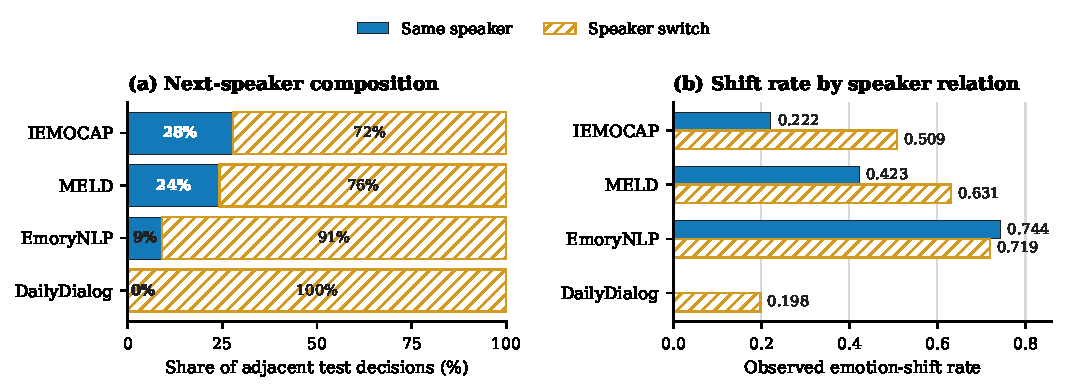
\includegraphics[width=0.96\textwidth]{figures/speaker_relation.pdf}
\caption{Speaker composition and emotion-shift rate at adjacent test decision points. Filled blue
bars denote same-speaker transitions; hatched bars denote speaker switches, preserving the
distinction in grayscale. DailyDialog has no adjacent same-speaker decisions. Exact denominators
are given in Table~\ref{tab:speaker}.}
\label{fig:speaker}
\end{figure*}

A 5{,}000-sample dialogue-cluster bootstrap confirms that the switch-minus-same shift-rate
difference is not merely an utterance-count artifact on IEMOCAP ($+0.287$, 95\% CI
$[+0.200,+0.373]$) or MELD ($+0.208$, $[+0.151,+0.265]$); both two-sided bootstrap
$p<.001$. EmoryNLP shows no supported difference ($-0.025$, $[-0.119,+0.072]$, $p=.614$).
DailyDialog cannot support this contrast because its same-speaker cell is empty. Resampling whole
dialogues is important here: treating 6{,}740 DailyDialog utterance pairs or 2{,}330 MELD pairs as
independent would understate clustered uncertainty.

The self-shift target also changes the effective sample and horizon. It removes the final
appearance of every speaker, leaving 80.0--98.1\% as many test decisions as the immediate target,
and its mean gap ranges from 1.98 to 2.51 turns. The shift-rate change is largest on IEMOCAP
(0.429 immediate to 0.263 self), confirming that the original aggregate rate partly reflects
cross-speaker contrast rather than within-person instability.

\begin{table}[t]
\centering
\footnotesize
\caption{Train-fold transition baselines under the two targets (test AUC). Global conditions only
on current emotion; speaker conditions on current emotion and speaker with sparse/unseen-speaker
backoff. These are label-only diagnostics, not learned-model results.}
\label{tab:selfbase}
\begin{tabular}{lcccc}
\toprule
& \multicolumn{2}{c}{Immediate} & \multicolumn{2}{c}{Self-shift} \\
Corpus & Global & Speaker & Global & Speaker \\
\midrule
IEMOCAP     & 0.642 & 0.642 & 0.586 & 0.586 \\
MELD        & 0.676 & 0.676 & 0.663 & 0.663 \\
EmoryNLP    & 0.608 & 0.608 & 0.592 & 0.592 \\
DailyDialog & 0.691 & 0.691 & 0.657 & 0.657 \\
\bottomrule
\end{tabular}
\end{table}

Table~\ref{tab:selfbase} shows that inertia remains predictive after redefining the target, but its
strength decreases on three corpora. Speaker conditioning contributes exactly zero AUC on every
corpus in this evaluation: IEMOCAP's global session-and-actor identities are genuinely unseen at
test time, and MELD, EmoryNLP, and DailyDialog roles are qualified by dialogue ID, so every
test-time speaker key is, by construction, absent from the train-fold speaker table and
the estimator always backs off to the global row. The baseline's full strength therefore comes
from the emotion-specific transition alone; this evaluation provides no evidence that
speaker-identity conditioning helps, only that dialogue-local role identities cannot be tested
for a within-person effect without a genuinely cross-dialogue speaker identifier.

Forecast horizon is another hidden source of heterogeneity. Table~\ref{tab:horizon} groups
self-shift decisions by the number of turns until the current speaker returns. IEMOCAP and MELD
show markedly higher shift rates after gaps of at least three turns than at gap one; EmoryNLP is
non-monotonic, and DailyDialog contains only gap-two decisions. A single aggregate self-shift score
therefore combines different horizons just as the immediate target combines different speaker
relations. Future benchmarks should either report horizon strata or define a fixed time/turn
horizon prospectively.

\begin{table}[t]
\centering
\footnotesize
\caption{Self-shift composition by forecast gap. Cells show test $N$ / shift rate; -- indicates
that the released test split contains no decision at that gap.}
\label{tab:horizon}
\begin{tabular}{lccc}
\toprule
Corpus & Gap 1 & Gap 2 & Gap $\geq3$ \\
\midrule
IEMOCAP     & 442 / .222 & 864 / .234 & 255 / .431 \\
MELD        & 565 / .423 & 961 / .580 & 338 / .612 \\
EmoryNLP    & 82 / .744  & 464 / .619 & 193 / .772 \\
DailyDialog & --         & 5{,}740 / .180 & -- \\
\bottomrule
\end{tabular}
\end{table}

\begin{table*}[t]
\centering
\footnotesize
\caption{Complete next-own-utterance self-shift ROC--AUC (three-seed mean). The full causal dialogue
history is retained; only the supervised target index changes. Trans-Pred is information-matched.
DailyDialog gains all survive the separate 24-comparison Holm correction ($p_{\rm adj}=.0048$);
other corrected comparisons are not significant.}
\label{tab:selfmodels}
\begin{tabular}{lccccccc}\toprule
Corpus & Trans-Pred & GRU & DRNN & DGCN & DAG-ERC & PEC & PseudoFut \\
\midrule
IEMOCAP     & .541 & .609 & .602 & .597 & .598 & .593 & .605 \\
MELD        & .584 & .593 & .600 & .608 & .610 & .593 & .593 \\
EmoryNLP    & .518 & .509 & .503 & .514 & .515 & .501 & .523 \\
DailyDialog & .577 & \textbf{.699} & \textbf{.706} & \textbf{.698} & \textbf{.691} & \textbf{.695} & \textbf{.693} \\
\bottomrule
\end{tabular}
\end{table*}

The self-shift benchmark supports a bounded generalization. DailyDialog remains the stable positive
case at the longer, exactly two-turn horizon ($+.114$ to $+.129$ AUC versus Trans-Pred). IEMOCAP
models are directionally positive but the test split contains only 31 dialogue clusters; MELD gains
are small, and EmoryNLP is tied. Redefining the target therefore changes both prevalence and model
evidence rather than merely renaming the original task.

\textbf{Main result (Table~\ref{tab:main}).} We evaluate a plain GRU, causal re-implementations of
DialogueRNN~\cite{majumder2019dialoguernn}, DialogueGCN~\cite{ghosal2019dialoguegcn}, and
DAG-ERC~\cite{shen2021dagerc}, plus PEC-style~\cite{altarawneh2023pec} and pseudo-future-style
forecasting strategies~\cite{xie2025pugcn}. Information matching changes the conclusion. In the
deployable regime, all six models exceed the train-only predicted-label transition baseline on
every primary text corpus in point estimate. The gain is decisive on duplicate-free DailyDialog
($+0.160$ to $+0.167$ ROC--AUC; all adjusted $p=.0144$) and smaller elsewhere. Among the primary
text corpora, DialogueRNN on MELD is the only other comparison that survives the 72-test
familywise correction ($\Delta=+0.041$, adjusted $p=.0352$); all six MELD-mm gains also survive
but sit in a feature-source sensitivity configuration rather than a primary corpus. Positive but
uncorrected differences on IEMOCAP and EmoryNLP are evidence of possible benefit, not conclusive
wins.

The oracle diagnostic asks a different question. When both sides receive gold $y_n$, all six
models remain clearly better on DailyDialog ($+0.106$ to $+0.132$; adjusted $p=.0144$), whereas
the transition baseline is stronger on MELD ($-0.032$ to $-0.064$), with four model differences
surviving correction. IEMOCAP is effectively tied and EmoryNLP is directionally favorable to the
baseline. Thus, the transition matrix is neither a universal lower bound nor a straw baseline:
its strength depends on whether current emotion is known and on corpus-specific transition
structure.

\textbf{Scope.} Four systems are causal, strategy-level re-implementations of representative ERC
families; PEC-style and pseudo-future-style are forecasting-inspired strategies. Our claims concern
evaluation practice and model families, not reproduction of any individual published score. The
MM-DFN feature release is a sensitivity analysis because its complete upstream producers are not
available; primary claims rest on four text corpora and are repeated using independently fitted,
strictly utterance-local text features. Finally, structural causality is verified rather than
inferred from architecture names: perturbing all inputs beyond the commitment point changes every
earlier logit by exactly zero for every tested implementation.

\begin{table*}[t]
\centering
\footnotesize
\caption{Deployable shift ROC--AUC (three-seed mean). Trans-Pred uses current-emotion predictions
from a train-only linear classifier; learned models receive no gold emotion. Bold values exceed the
matched baseline. DailyDialog is duplicate-free. MM rows are feature-source sensitivity analyses,
not independent primary corpora. Inference uses a seed--dialogue hierarchical bootstrap and paired
dialogue-cluster permutation; Holm correction spans 72 declared deployable+oracle comparisons.
All six DailyDialog gains, all six MELD-mm gains, and DialogueRNN's MELD gain survive correction.}
\label{tab:main}
\begin{tabular}{lccccccc}\toprule
Dataset & Trans-Pred & GRU & DRNN & DGCN & DAG-ERC & PEC & PseudoFut \\
\midrule
IEMOCAP      & .576 & \textbf{.647} & \textbf{.627} & \textbf{.609} & \textbf{.607} & \textbf{.632} & \textbf{.631} \\
MELD         & .588 & \textbf{.621} & \textbf{.629} & \textbf{.623} & \textbf{.608} & \textbf{.620} & \textbf{.600} \\
EmoryNLP     & .501 & \textbf{.521} & \textbf{.533} & \textbf{.536} & \textbf{.554} & \textbf{.539} & \textbf{.542} \\
DailyDialog  & .580 & \textbf{.746} & \textbf{.744} & \textbf{.748} & \textbf{.744} & \textbf{.743} & \textbf{.741} \\
IEMOCAP-mm   & .566 & .560 & \textbf{.598} & \textbf{.593} & .559 & \textbf{.581} & \textbf{.578} \\
MELD-mm      & .584 & \textbf{.723} & \textbf{.716} & \textbf{.724} & \textbf{.720} & \textbf{.720} & \textbf{.723} \\
\bottomrule
\end{tabular}
\end{table*}

\begin{table*}[t]
\centering
\footnotesize
\caption{Oracle information-matched shift ROC--AUC (three-seed mean). Both the transition baseline
and every learned model receive gold current emotion. Bold values exceed Trans-Gold. DailyDialog
and MELD-mm gains survive joint Holm correction; on MELD, four of the six negative differences
survive.}
\label{tab:oracle}
\begin{tabular}{lccccccc}\toprule
Dataset & Trans-Gold & GRU & DRNN & DGCN & DAG-ERC & PEC & PseudoFut \\
\midrule
IEMOCAP      & .642 & \textbf{.649} & .615 & .617 & .616 & .631 & .610 \\
MELD         & .676 & .630 & .629 & .628 & .644 & .632 & .612 \\
EmoryNLP     & .608 & .553 & .561 & .561 & .563 & .591 & .525 \\
DailyDialog  & .694 & \textbf{.808} & \textbf{.820} & \textbf{.826} & \textbf{.822} & \textbf{.804} & \textbf{.800} \\
IEMOCAP-mm   & .642 & .566 & .590 & .598 & .577 & .594 & .569 \\
MELD-mm      & .676 & \textbf{.802} & \textbf{.791} & \textbf{.805} & \textbf{.807} & \textbf{.798} & \textbf{.798} \\
\bottomrule
\end{tabular}
\end{table*}

Tables~\ref{tab:main} and~\ref{tab:oracle} average three independently trained seeds; inference
uses all three raw score vectors rather than a single representative run. The strongest primary
result is therefore not merely numerical: on DailyDialog every model has a positive delta in every
seed, the 95\% hierarchical intervals exclude zero, and all paired permutation tests remain
significant after the declared joint correction.

\textbf{Implementation corrections.} The audit found and repaired two defects before the revised
experiment was declared: PEC recency weights were reversed, and pseudo-future auxiliary MSE
included padded positions. Separate cache namespaces retain historical runs for traceability, but
Tables~\ref{tab:main}--\ref{tab:oracle}, all inference, and all supplementary controls use only the
corrected implementations.

\textbf{Independent utterance-local features.} Table~\ref{tab:feat} removes dependence on released
deep embeddings. TF--IDF vocabulary and IDF, followed by rank-128 truncated SVD, are fitted only on
training utterances; each utterance is then transformed independently with finite-value checks.
The local-feature GRU remains substantially above its matched predicted-label transition baseline
on IEMOCAP and DailyDialog and directionally above it on EmoryNLP; MELD is tied. Absolute AUC is
lower than with RoBERTa on three corpora, as expected for a shallow representation. Crucially, the
DailyDialog advantage is unchanged in magnitude ($+.164$ versus $+.166$ with RoBERTa), so its
headline improvement cannot be attributed solely to unobserved context in an upstream encoder.
The mixed pattern also cautions against treating any released feature source as architecture-neutral.

\begin{table}[t]
\centering
\footnotesize
\caption{Strict utterance-local feature control (three-seed ROC--AUC). Both the GRU features and
the baseline's current-emotion classifier are refit from the same train-only TF--IDF/SVD rows.
Intervals and $p$-values use the same seed--dialogue procedures as the main experiment.}
\label{tab:feat}
\begin{tabular}{lccc}
\toprule
Corpus & GRU & Trans-Pred & $\Delta$ [95\% CI] \\
\midrule
IEMOCAP     & .642 & .552 & +.089 [.010,.154] \\
MELD        & .539 & .538 & +.001 [-.027,.028] \\
EmoryNLP    & .555 & .494 & +.061 [.014,.112] \\
DailyDialog & .673 & .509 & +.164 [.141,.185] \\
\bottomrule
\end{tabular}
\end{table}

\textbf{Same-architecture dose response (Fig.~\ref{fig:dose}).} A single-layer Transformer holds
parameters, positional encoding, pooling, optimizer, and checkpoint rule fixed; only its attention
mask changes so that position $n$ sees $k\in\{0,1,2,4,\mathrm{all}\}$ future utterances. A single
layer is required for $k$ to mean what the sweep claims: with a stacked multi-layer encoder using
the same window mask at every layer, a later layer's query at $n$ can read an earlier layer's
output at $n+k$, which already mixed in $x_{n+2k}$, giving an effective receptive field of
${\sim}Lk$ for $L$ layers rather than $k$. The response is not monotone. MELD rises from .620 at
$k=0$ to .685 at $k=1$, then falls to .651/.637/.632. Duplicate-free DailyDialog similarly rises
from .736 to .780 and falls to .774/.758/.751. The other four configurations vary by at most .022
without a consistent direction. Thus, exposure to the target utterance can materially inflate
performance, but additional future context need not add signal and may dilute or complicate
optimization. Because architecture is held fixed and the receptive field is exactly $k$, this
conclusion no longer relies on comparing a look-ahead GRU with a bidirectional GRU, nor on a
multi-layer encoder whose effective receptive field exceeds its nominal window.

\begin{figure*}[t]
\centering
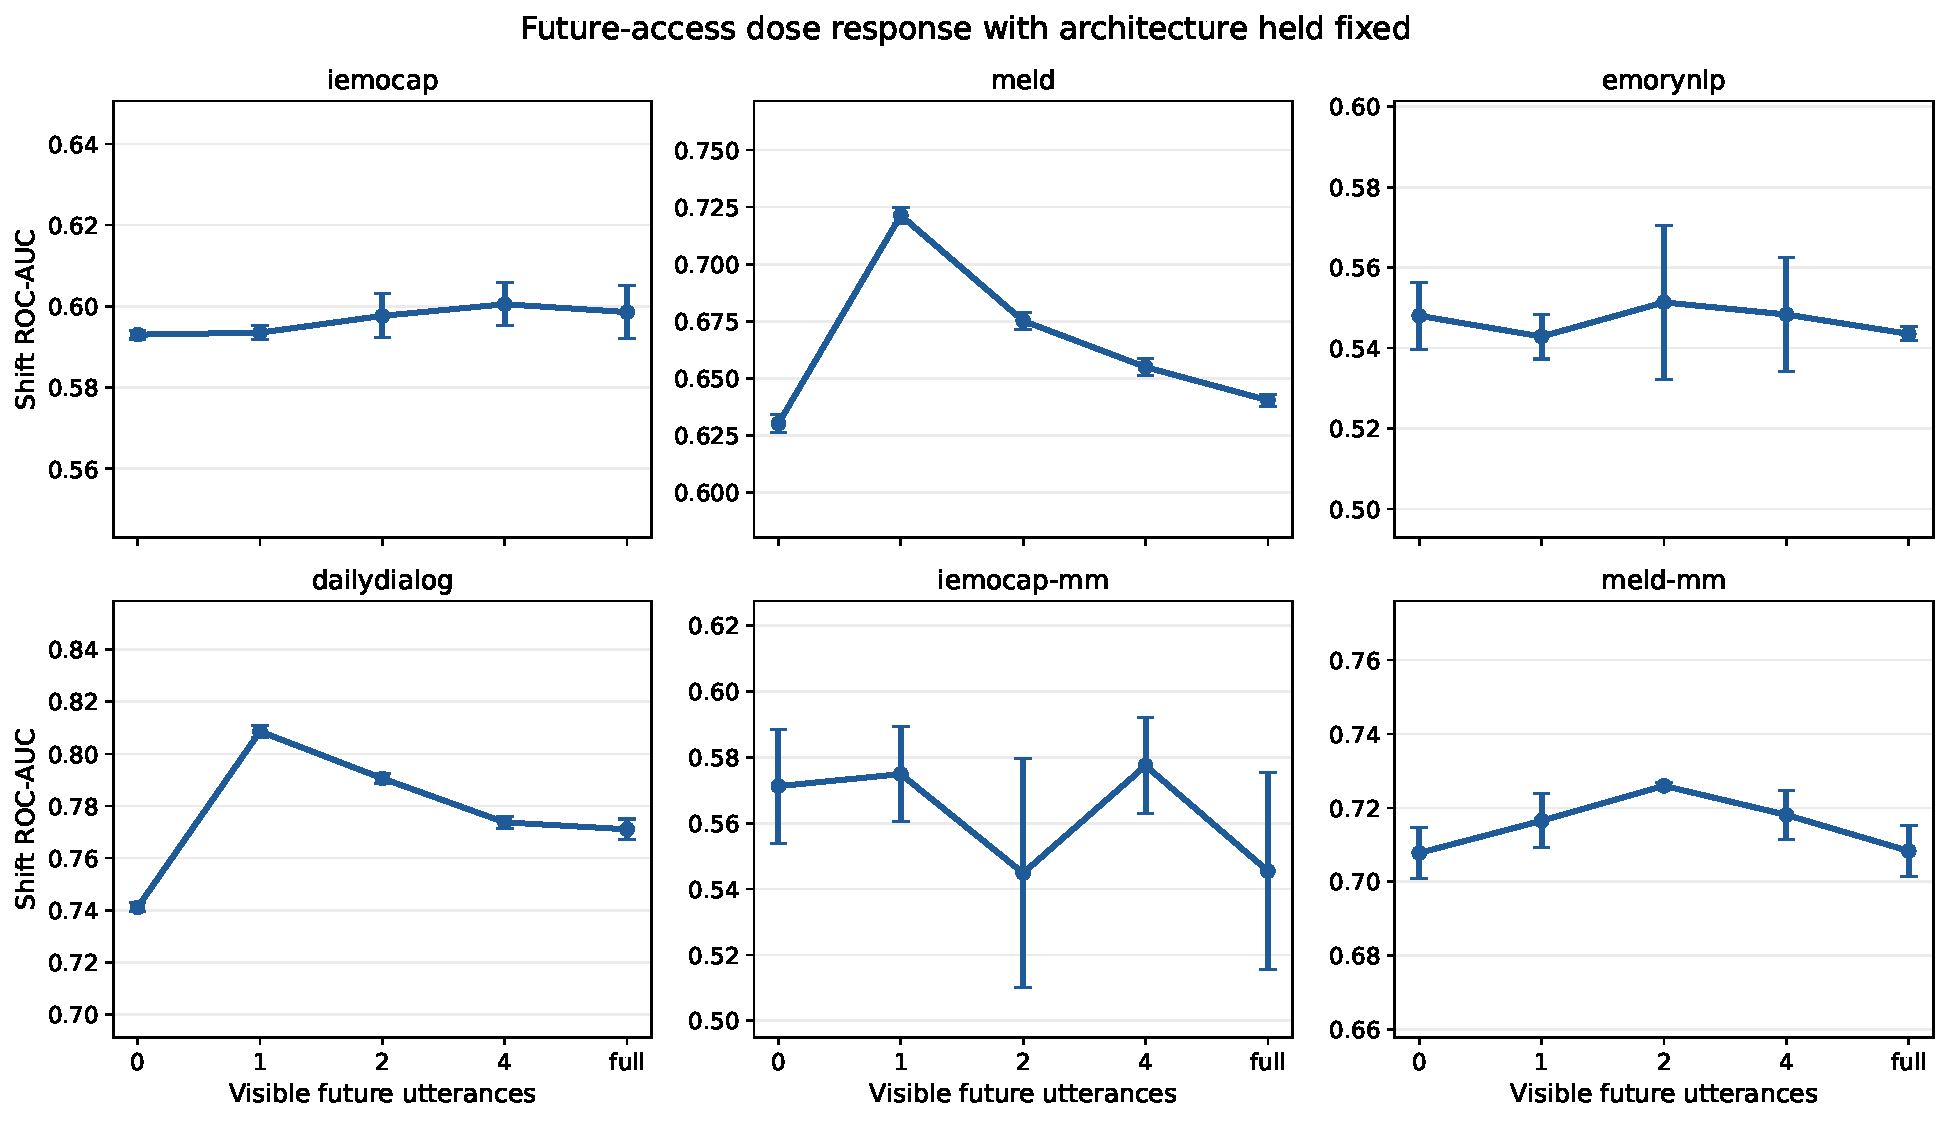
\includegraphics[width=0.96\textwidth]{figures/leakage_uniform_transformer.pdf}
\caption{Future-access dose response with one fixed Transformer architecture. Error bars show
three-seed standard deviation. MELD and DailyDialog peak when the target utterance alone becomes
visible; none of the six configurations supports a general monotonic-more-future claim.}
\label{fig:dose}
\end{figure*}

\subsection{Split and Leakage Robustness}
\label{sec:robust}

\textbf{Exact dialogue contamination.} We hashed each dialogue by its complete ordered utterance
text and compared validation/test hashes against the training fold (Table~\ref{tab:duplicates}).
IEMOCAP and EmoryNLP contain no exact cross-fold matches; MELD contains one duplicate test
dialogue; DailyDialog contains 134/1{,}000 duplicate test dialogues and 101/1{,}000 duplicate
validation dialogues. This is a corpus property visible before model fitting, not a model-specific
leak, but it can make a positive result look stronger.

\begin{table}[t]
\centering
\footnotesize
\caption{Exact train-fold dialogue duplicates. A duplicate has an identical full ordered text
sequence, not merely an overlapping utterance.}
\label{tab:duplicates}
\begin{tabular}{lrrrr}
\toprule
& \multicolumn{2}{c}{Test} & \multicolumn{2}{c}{Validation} \\
Corpus & $N$ & Dup. & $N$ & Dup. \\
\midrule
IEMOCAP     & 31    & 0   & 12    & 0 \\
MELD        & 280   & 1   & 114   & 0 \\
EmoryNLP    & 79    & 0   & 89    & 0 \\
DailyDialog & 1{,}000 & 134 & 1{,}000 & 101 \\
\bottomrule
\end{tabular}
\end{table}

We remove every matching DailyDialog validation/test dialogue before any configuration search,
checkpoint selection, baseline fitting, or reported evaluation. Test dialogues fall from 1,000 to
866 and validation dialogues from 1,000 to 899. All DailyDialog results in this paper---main,
oracle, state-factorized, local-feature, self-shift, and dose-response---use this same clean split.

Earlier unequal-architecture look-ahead controls are retained in the repository for historical
traceability but are not used for the revised leakage claim; Fig.~\ref{fig:dose} supersedes them by
holding architecture and parameter count fixed.

\vspace{-2mm}\section{Findings and Discussion}

The revised evidence supports six bounded findings.

\begin{enumerate}
\item Information matching is consequential. No-label models consistently exceed a baseline fed
noisy train-only label predictions in point estimate, whereas a gold-label transition matrix is
competitive or stronger on several corpora.
\item DailyDialog is the most stable positive case: every tested model beats both matched baselines
after duplicate removal, across every seed, with corrected-significant hierarchical inference.
\item MELD is conditional: learned models improve on the deployable predicted-label baseline, but
most lose to the oracle gold-label baseline. The current-state observation, not only architecture,
changes the answer.
\item Ranking and probability quality diverge. PR--AUC corroborates DailyDialog discrimination,
while Brier/ECE show that learned scores require calibration before risk interpretation.
\item Feature provenance remains part of the estimand. The independently fitted local-feature
control preserves large DailyDialog and IEMOCAP gains, but not the MELD gain.
\item Adjacent-turn shift is predominantly cross-speaker in all four corpora; interaction-level
next-turn shift and a person's next-own-utterance self-shift are distinct targets and are evaluated
separately here.
\end{enumerate}

These findings do not establish that one architecture class is generally superior or irrelevant.
They establish a narrower measurement result: the sign and magnitude of model-versus-transition
differences depend on the information supplied to both sides, and conclusions that omit this
factor can reverse. Architecture spreads within a configuration are often modest, but the equal
search is intentionally limited and the systems are causal re-implementations. Larger searches or
new forecasting-native systems may change their ordering.

The multimodal rows reinforce the need for restraint. Their point estimates can be large, but the
complete upstream producers are unavailable and repeated identical MELD strings do not always map
to identical released vectors. They are therefore useful sensitivity evidence, not the basis for a
claim that a modality or representation is intrinsically better. The independently generated local
control supplies the stronger provenance test.

\subsection{What the Speaker Audit Changes}

The audit in \S\ref{sec:speaker} changes the language appropriate for the task. The immediate
target is not ``will this person change emotion on their next turn?'' unless evaluation is
restricted to $s_{n+1}=s_n$. It is ``will the emotion expressed by the conversation's next
utterance differ from the current utterance?'' This remains meaningful for a dialogue manager that
cares about the next observed affect regardless of speaker, but it combines within-person dynamics
with cross-person response dynamics.

The distinction also clarifies the transition result. A model can exploit emotion persistence,
common cross-speaker response pairs, or a correlation between turn-taking and label change. The
last signal is available at commitment time only if the next speaker is scheduled or otherwise
known. Our headline models are not given $s_{n+1}$, so the stratified rates are explanatory
diagnostics rather than an oracle input. Future benchmarks should state whether next-speaker
identity is known and, if so, provide it symmetrically to learned models and baselines.

\subsection{Operational Implications}

Temporal validity is necessary but not sufficient for deployment. A high-AUC alert can still be
poorly calibrated, too late for intervention, or unfairly concentrated on particular speakers.
The commitment point must correspond to a real action window: after the current turn is available
but before any acoustic, lexical, or metadata trace of the next turn enters the system. Production
logs should retain feature timestamps so this boundary remains auditable.

Thresholds should follow intervention costs rather than F1 alone. In de-escalation, a false
negative may miss harm while repeated false positives create alert fatigue. AUC supports model
comparison but does not select an operating point; calibration, precision--recall tradeoffs, and
cost-sensitive validation are needed before use. This distinction is visible in the strongest
ranking result: duplicate-free DailyDialog DialogueGCN reaches ROC--AUC .748 and PR--AUC .441,
but its uncalibrated Brier score/ECE are .188/.224, versus .153/.052 for the weaker predicted-label
transition baseline. Post-hoc calibration must therefore be fitted on held-out deployment-like
data before probabilities are interpreted as risks. Emotion labels also concern sensitive and
culturally ambiguous human states. This work audits measurement; it does not establish that an
automated emotional intervention is safe or appropriate.

\subsection{Threats to Validity and Limitations}

\textbf{Construct validity.} Emotion annotations are discrete expressions, not direct measures of
internal affect. Both targets inherit annotator disagreement and collapse different transition
types into one event. The self-shift benchmark is complete across the six tested model families,
but it changes both the target horizon and sample composition and should not be read as a direct
ranking against immediate-shift scores.

\textbf{Internal validity.} Causality tests cover model forward paths, masks, and provided feature
arrays, but cannot retroactively certify every upstream feature-extraction step. COSMIC producer
code directly supports utterance-local extraction for three corpora; DailyDialog is supported by
schema/output checks, while MM-DFN is not certified to the same level. The train-only TF--IDF/SVD
control reduces, but cannot remove, construct limitations from discrete emotion labels and splits.

\textbf{Split validity.} We remove exact train--test dialogue duplication from every DailyDialog
headline and supplementary run, but not subtler writing-style leakage. MELD, EmoryNLP, and DailyDialog identities
in the released pickles are dialogue-local, not verified global persons. Only IEMOCAP's session
split provides an unseen-actor test. Speaker conditioning elsewhere means local role conditioning,
not person-level generalization.

\textbf{Statistical validity.} Three seeds characterize optimization variability but do not make
the six configurations independent: two corpora recur under different feature sources. Joint Holm
correction is intentionally conservative. Hierarchical intervals and paired permutation tests use
all seeds and whole-dialogue clusters, but neither procedure replaces replication on a
prospectively designed forecasting corpus.

\textbf{Model scope.} Forecasting-specific systems are strategy-level re-implementations because
original code was unavailable; we do not claim every detail of a named publication. The common
four-configuration search favors comparability over per-model best-case tuning and does not span
architecture-specific graph windows or all loss families. Any larger search should apply the same
budget to competing families and retain validation-only selection.

\textbf{Information matching is imperfect in both directions.} In the oracle diagnostic, the gold
one-hot label is concatenated to the per-turn feature vector at every position $t \le n$, so a
sequential or attention-based model's representation at $n$ is conditioned on the entire observed
label history $y_1,\ldots,y_n$, not on $y_n$ alone; the transition baseline, by construction,
conditions only on the single most recent label. ``Information-matched'' therefore means matched
at the single quantity the title foregrounds -- current-emotion availability -- not matched in
the total label information reaching each side, and the oracle gap likely understates the
transition baseline's competitiveness under a strict single-label match. Symmetrically, the
deployable regime's transition baseline consumes a hard current-label prediction from a linear
classifier rather than the classifier's posterior, discarding calibrated uncertainty that a
posterior-marginalized or cross-fitted baseline could exploit; this is a conservative choice for
our headline claim (a stronger predicted-label baseline could only narrow, not widen, the
learned-model advantage we report), but it means the deployable comparison is not the strongest
baseline we could construct. Both limitations bound the oracle and deployable comparisons in
opposite directions and are left as reporting caveats rather than resolved with a new baseline
family in this submission.

\section{Reproducibility Artifacts}
\label{sec:artifact}

The repository is organized so each major claim has an executable producer rather than being a
manually assembled table. Table~\ref{tab:artifact} maps the paper's evidence to source and output
artifacts. Feature pickles are not redistributed because of size and upstream licensing; the
README records expected filenames and provenance. Every result script is resumable through
dataset-specific JSON caches, and historical caches are kept separate from revised experiment
caches.

\begin{table*}[t]
\centering
\scriptsize
\caption{Claim-to-artifact map. Producers are under \texttt{src/}; reviewable outputs are under
\texttt{results/}.}
\label{tab:artifact}
\begin{tabular}{lll}
\toprule
Claim & Producer & Reviewable output \\
\midrule
Main benchmark & \texttt{access\_revision\_experiments} & JSON/Markdown + raw scores \\
Structural causality & \texttt{check\_causality} & causality check \\
Uniform leakage dose & \texttt{access\_uniform\_dose\_response} & figure + JSON \\
Joint inference & \texttt{evaluate}, \texttt{holm\_correction} & 72 corrected tests \\
Speaker audit & \texttt{access\_speaker\_analysis} & target/stratum JSON \\
Full self-shift & \texttt{access\_self\_shift\_benchmark} & six-model raw scores \\
Local feature control & \texttt{access\_local\_feature\_control} & train-only features/results \\
Data/provenance audit & \texttt{access\_data\_quality} & alignment/integrity report \\
\bottomrule
\end{tabular}
\end{table*}

The minimum reproduction sequence is to place the released features under \texttt{data/feat}, run
the data-quality and causality modules, and then run the primary revision module; exact commands
are in the packaged README. Supplementary producers use isolated cache namespaces and resume from
completed seeds. The paper source includes the IEEE Access class, fonts, figures, and a compiled
PDF matching the submitted \LaTeX{} source.

\vspace{-3mm}\section{Minimal Reporting Checklist}

Standalone checklist for future EFC-forecasting papers: (1) state the commitment point and verify
no feature crosses it; (2) name the semantic target---interaction-level next turn or same-person
next own turn---and report speaker-relation composition; (3) verify causality directly (e.g.\ a
future-perturbation test), not by architecture claim alone; (4) trace feature provenance upstream
of the classifier; (5) match current-label information between learned models and train-only
transition baselines; (6) report ROC--AUC, PR--AUC, calibration, balanced accuracy, and prediction
rate rather than F1 alone; (7) use seed--dialogue-aware paired inference corrected jointly across
the declared comparison family; (8) label leaky ablations and exclude them from headline
comparisons; (9) check duplicate dialogues and global speaker overlap; and (10) release masks,
split identifiers, raw seed-level predictions, and audit logs.

\vspace{-3mm}\section{Conclusion}

Information-matched evaluation changes the interpretation of conversational emotion-shift
forecasting. Models that receive no gold current label can meaningfully outperform a transition
baseline driven by train-only predicted labels; on duplicate-free DailyDialog this conclusion is
large, seed-consistent, and familywise significant. A transition matrix supplied with gold current
emotion is nevertheless competitive on IEMOCAP and stronger on MELD, showing why privileged-label
diagnostics must not be presented as deployable comparisons. Independent local features preserve
the DailyDialog result, while calibration metrics warn that strong ranking is not yet reliable risk
estimation. Finally, adjacent interaction shift and same-person self-shift are both legitimate but
different targets requiring explicit horizons and matched baselines. The general lesson is
methodological rather than architectural: state the temporal, information, provenance, and semantic
contracts before interpreting a model comparison~\cite{kapoor2023leakage,dacrema2019recsys,lin2019neuralhype}.
The submission supplement contains executable producers, locked environment files, checksums, and
raw seed predictions. The public project page is
\url{https://github.com/GawaineXiukkie/emotion-forecasting-leakage-audit}; an immutable release tag
will be created from the final reviewed artifact before the reproducibility claim is made public.

\section*{Acknowledgment}

The authors used OpenAI Codex to assist with English-language editing, \LaTeX{} formatting, code
review, and the preparation of supplementary analyses. The authors reviewed and verified the
manuscript, code changes, experimental results, and conclusions and assume full responsibility
for the submitted work.

\begin{thebibliography}{00}

\bibitem{poria2019meld} S. Poria, D. Hazarika, N. Majumder, G. Naik, E. Cambria, and R. Mihalcea,
``MELD: A multimodal multi-party dataset for emotion recognition in conversations,'' in
\emph{Proc. ACL}, 2019, pp. 527--536.

\bibitem{busso2008iemocap} C. Busso, M. Bulut, C.-C. Lee, A. Kazemzadeh, E. Mower, S. Kim, J. N.
Chang, S. Lee, and S. S. Narayanan, ``IEMOCAP: Interactive emotional dyadic motion capture
database,'' \emph{Language Resources and Evaluation}, vol. 42, no. 4, pp. 335--359, 2008.

\bibitem{zahiri2018emorynlp} S. M. Zahiri and J. D. Choi, ``Emotion detection on TV show
transcripts with sequence-based convolutional neural networks,'' in \emph{Proc. AAAI Workshop},
2018.

\bibitem{li2017dailydialog} Y. Li, H. Su, X. Shen, W. Li, Z. Cao, and S. Niu, ``DailyDialog: A
manually labelled multi-turn dialogue dataset,'' in \emph{Proc. IJCNLP}, 2017, pp. 986--995.

\bibitem{ghosal2020cosmic} D. Ghosal, N. Majumder, A. Gelbukh, R. Mihalcea, and S. Poria, ``COSMIC:
Commonsense knowledge for emotion identification in conversations,'' in \emph{Findings of EMNLP},
2020, pp. 2470--2481.

\bibitem{hu2021mmdfn} D. Hu, X. Hou, L. Wei, L. Jiang, and Y. Mo, ``MM-DFN: Multimodal dynamic
fusion network for emotion recognition in conversations,'' in \emph{Proc. ICASSP}, 2022.

\bibitem{majumder2019dialoguernn} N. Majumder, S. Poria, D. Hazarika, R. Mihalcea, A. Gelbukh, and
E. Cambria, ``DialogueRNN: An attentive RNN for emotion detection in conversations,'' in
\emph{Proc. AAAI}, 2019, pp. 6818--6825.

\bibitem{ghosal2019dialoguegcn} D. Ghosal, N. Majumder, S. Poria, N. Chhaya, and A. Gelbukh,
``DialogueGCN: A graph convolutional neural network for emotion recognition in conversation,'' in
\emph{Proc. EMNLP-IJCNLP}, 2019, pp. 154--164.

\bibitem{shen2021dagerc} W. Shen, S. Wu, Y. Yang, and X. Quan, ``Directed acyclic graph network for
conversational emotion recognition,'' in \emph{Proc. ACL-IJCNLP}, 2021.

\bibitem{ai2023dergcn} W. Ai, Y. Shou, T. Meng, and K. Li, ``DER-GCN: Dialogue and event
relation-aware graph convolutional neural network for multimodal dialogue emotion recognition,''
\emph{arXiv:2312.10579}, 2023.

\bibitem{zhong2019ket} P. Zhong, D. Wang, and C. Miao, ``Knowledge-enriched transformer for emotion
detection in textual conversations,'' in \emph{Proc. EMNLP-IJCNLP}, 2019, pp. 165--176.

\bibitem{hu2021dialoguecrn} D. Hu, L. Wei, and X. Huai, ``DialogueCRN: Contextual reasoning
networks for emotion recognition in conversations,'' in \emph{Proc. ACL-IJCNLP}, 2021.

\bibitem{hazarika2018icon} D. Hazarika, S. Poria, R. Mihalcea, E. Cambria, and R. Zimmermann,
``ICON: Interactive conversational memory network for multimodal emotion detection,'' in
\emph{Proc. EMNLP}, 2018, pp. 2594--2604.

\bibitem{tsai2019mult} Y.-H. H. Tsai, S. Bai, P. P. Liang, J. Z. Kolter, L.-P. Morency, and R.
Salakhutdinov, ``Multimodal Transformer for unaligned multimodal language sequences,'' in
\emph{Proc. ACL}, 2019, pp. 6558--6569.

\bibitem{hu2021mmgcn} J. Hu, Y. Liu, J. Zhao, and Q. Jin, ``MMGCN: Multimodal fusion via deep graph
convolution network for emotion recognition in conversation,'' in \emph{Proc. ACL-IJCNLP}, 2021,
pp. 5666--5675.

\bibitem{hazarika2020misa} D. Hazarika, R. Zimmermann, and S. Poria, ``MISA: Modality-invariant and
-specific representations for multimodal sentiment analysis,'' in \emph{Proc. ACM MM}, 2020, pp.
1122--1131.

\bibitem{li2023ga2mif} J. Li, X. Wang, G. Lv, and Z. Zeng, ``GA2MIF: Graph and attention based
two-stage multi-source information fusion for conversational emotion detection,'' \emph{IEEE
Trans. Affective Computing}, vol. 15, no. 1, pp. 130--143, 2023.

\bibitem{meng2024mglra} T. Meng, F. Zhang, Y. Shou, H. Shao, W. Ai, and K. Li, ``Masked graph
learning with recurrent alignment for multimodal emotion recognition in conversation,''
\emph{IEEE/ACM Trans. Audio, Speech, Lang. Process.}, vol. 32, pp. 4298--4312, 2024.

\bibitem{wang2024hief} H. Wang, X. Mai, Z. Tao, J. Lin, X. Tong, I. Pan, S. Yan, Y. Wang, and S.
Gao, ``Hi-EF: Benchmarking emotion forecasting in human-interaction,'' \emph{arXiv:2407.16406},
2024.

\bibitem{altarawneh2023pec} E. Altarawneh, A. Agrawal, M. Jenkin, and M. Papagelis, ``Predicting
evoked emotions in conversations,'' \emph{arXiv:2401.00383}, 2023.

\bibitem{shi2023epc} X. Shi, X. Li, and T. Toda, ``Emotion awareness in multi-utterance turn for
improving emotion prediction in multi-speaker conversation,'' in \emph{Proc. Interspeech}, 2023,
pp. 765--769.

\bibitem{shi2024epc} H. Shi, Z. Liang, and J. Yu, ``Emotional cues extraction and fusion for
multi-modal emotion prediction and recognition in conversation,'' in \emph{Proc. Interspeech},
2024, pp. 4074--4078.

\bibitem{ju2023mrepc} X. Ju, D. Zhang, S. Zhu, J. Li, S. Li, and G. Zhou, ``Real-time emotion
pre-recognition in conversations with contrastive multi-modal dialogue pre-training,'' in
\emph{Proc. ACM CIKM}, 2023.

\bibitem{xie2025pugcn} Y. Xie, Y. Liu, C. Sun, \emph{et al.}, ``Pseudo-utterance-guided contrastive
network for emotion forecasting in conversations,'' \emph{Expert Systems with Applications}, vol.
279, p. 127382, 2025.

\bibitem{lu2023edfc} X. Lu, W. Zhao, Y. Zhao, B. Qin, Z. Zhang, and J. Wen, ``A topic-enhanced
approach for emotion distribution forecasting in conversations,'' in \emph{Proc. IEEE ICASSP},
2023.

\bibitem{debsharma2025erfc} A. Debsharma, B. Jagyasi, S. Sen, P. Pandey, D. Dovari, V. C. Yuvaraj,
R. Parida, and G. Contractor, ``ERFC: Happy customers with emotion recognition and forecasting in
conversation in call centers,'' \emph{arXiv:2509.18175}, 2025.

\bibitem{gao2022esderc} Q. Gao, B. Cao, X. Guan, T. Gu, X. Bao, J. Wu, B. Liu, and J. Cao, ``Emotion
recognition in conversations with emotion shift detection based on multi-task learning,''
\emph{Knowledge-Based Systems}, vol. 248, p. 108861, 2022.

\bibitem{li2024cfnesa} J. Li, Y. Liu, X. Wang, and Z. Zeng, ``CFN-ESA: A cross-modal fusion network
with emotion-shift awareness for dialogue emotion recognition,'' \emph{IEEE Trans. Affective
Computing}, vol. 15, no. 4, pp. 1919--1933, 2024.

\bibitem{nirujan2025emoshiftnet} H. Nirujan and Y. H. P. P. Priyadarshana, ``EmoShiftNet: A
shift-aware multi-task learning framework with fusion strategies for emotion recognition in
multi-party conversations,'' \emph{Frontiers in Artificial Intelligence}, vol. 8, p. 1618698, 2025.

\bibitem{kumar2023efr} S. Kumar, S. Dudeja, M. S. Akhtar, and T. Chakraborty, ``Emotion flip
reasoning in multi-party conversations,'' \emph{IEEE Trans. Artificial Intelligence},
\emph{arXiv:2306.13959}, 2023.

\bibitem{kumar2024ediref} S. Kumar, M. S. Akhtar, E. Cambria, and T. Chakraborty, ``SemEval-2024
Task 10: Emotion discovery and reasoning its flip in conversation (EDiReF),'' in \emph{Proc. 18th
SemEval}, 2024, pp. 1933--1946.

\bibitem{kapoor2023leakage} S. Kapoor and A. Narayanan, ``Leakage and the reproducibility crisis in
machine-learning-based science,'' \emph{Patterns}, vol. 4, no. 9, p. 100804, 2023.

\bibitem{dacrema2019recsys} M. Ferrari Dacrema, P. Cremonesi, and D. Jannach, ``Are we really
making much progress? A worrying analysis of recent neural recommendation approaches,'' in
\emph{Proc. ACM RecSys}, 2019, pp. 101--109.

\bibitem{lin2019neuralhype} J. Lin, ``The neural hype and comparisons against weak baselines,''
\emph{ACM SIGIR Forum}, vol. 52, no. 2, pp. 40--51, 2019.

\bibitem{saito2015pr} T. Saito and M. Rehmsmeier, ``The precision--recall plot is more informative
than the ROC plot when evaluating binary classifiers on imbalanced datasets,'' \emph{PLoS ONE},
vol. 10, no. 3, p. e0118432, 2015.

\bibitem{guo2017calibration} C. Guo, G. Pleiss, Y. Sun, and K. Q. Weinberger, ``On calibration of
modern neural networks,'' in \emph{Proc. 34th Int. Conf. Machine Learning}, 2017, pp. 1321--1330.

\bibitem{saravanan2020bootstrap} V. Saravanan, G. J. Berman, and S. J. Sober, ``Application of the
hierarchical bootstrap to multi-level data in neuroscience,'' \emph{Neuron, Behavior, Data
Analysis, and Theory}, vol. 3, no. 5, 2020.

\end{thebibliography}

\begin{IEEEbiography}[{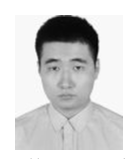
\includegraphics[width=1in,height=1.25in,clip,keepaspectratio]{author_photos/bin_wen.png}}]{Bin Wen}
received the B.Eng. degree in software engineering from Southern College of Sun Yat-sen
University, Guangzhou, China, in 2023. He is currently pursuing the M.Sc. degree in computer
science with Universiti Sains Malaysia, George Town, Malaysia.

His current research interests include multimodal sentiment analysis, multimodal large language
models, affective computing, speech enhancement, conversational emotion forecasting, and
human-computer interaction. His work focuses on parameter-efficient adaptation, discriminative
hidden-state readout, multimodal fusion, efficient speech enhancement, controlled comparisons,
ablation studies, and benchmark evaluation.
\end{IEEEbiography}

\begin{IEEEbiography}[{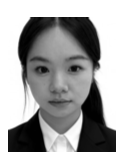
\includegraphics[width=1in,height=1.25in,clip,keepaspectratio]{author_photos/dai_qiao_zhang.png}}]{Dai-Qiao Zhang}
received the B.S. degree in mathematics and applied mathematics from Jimei University, China, in
2024. She is currently pursuing the Master's degree with the School of Mathematical Sciences,
Universiti Sains Malaysia.

Her research interests include topological data analysis and educational data mining.
\end{IEEEbiography}

\begin{IEEEbiography}[{
\includegraphics[width=1in,height=1.25in,clip,keepaspectratio]{author_photos/tien_ping_tan.png}}]{Tien-Ping Tan}
received the Ph.D. degree from Universit\'e Joseph Fourier, France, in 2008. He is currently an
Associate Professor with the School of Computer Sciences, Universiti Sains Malaysia, George Town,
Malaysia.

His research interests include automatic speech recognition, machine translation, and natural
language processing. Dr. Tan is the corresponding author of this article.
\end{IEEEbiography}

\EOD
\end{document}
